
The data provided by PAN consists of 420 XML files, where each file is named for the user ID and contains 200 tweets. The tweets are anonymized, so hashtag, user and URL information is replaced by generic tags. Another file contains the author ID's and the ground truth labels -- either I (ironic) or NI (non-ironic). The data is balanced. 
%balanced

\begin{figure*}[!h]
    \centering
    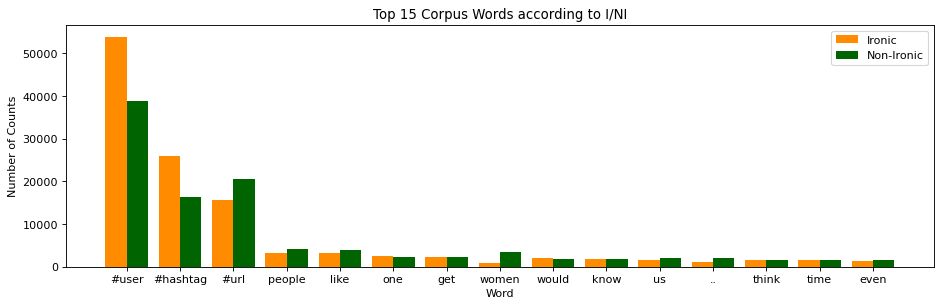
\includegraphics[width=\textwidth]{images/word_counts_i_ni.png}
    \caption{Bar plots for the top 20 most used words in the corpus according to the two classes.}
    \label{fig:bar_word_counts}
\end{figure*}

\subsection{Challenges of Data}

In manual irony annotation of tweets, \citeA{van2018exploring} found that among ironic tweets realized through polarity contrast (71\% of all ironic tweets), half were only identifiable as such by hashtag use. This means that absence of hashtags in the data will likely increase the difficulty of the task (see also \citeA{maynard2014hashtag} on hashtag-based classification). 

Another limitation of the dataset is the fact that we have no way of accessing conversational context for reply tweets, which has been shown to be significant for identifying irony \cite{joshi2015harnessing, wallace2015sparse}. Single tweets and reply tweets are treated the same in the dataset, even though we might expect that irony would function differently for them. 

\subsection{Data Pre-Processing}

% do we also remove the hashtag tags?
Our pre-processing methods are dependent on which features are being generated. However, for most features we remove the generic hashtag, user and URL tags from the tweets before processing them. These are then tokenized by the \emph{TweetTokenizer} provided by NLTK\footnote{\url{https://www.nltk.org/api/nltk.tokenize.casual.html}}. This is optimized to capture smileys and long words which are not standard English. 